\documentclass[twoside]{book}

% Packages required by doxygen
\usepackage{fixltx2e}
\usepackage{calc}
\usepackage{doxygen}
\usepackage[export]{adjustbox} % also loads graphicx
\usepackage{graphicx}
\usepackage[utf8]{inputenc}
\usepackage{makeidx}
\usepackage{multicol}
\usepackage{multirow}
\PassOptionsToPackage{warn}{textcomp}
\usepackage{textcomp}
\usepackage[nointegrals]{wasysym}
\usepackage[table]{xcolor}

% Font selection
\usepackage[T1]{fontenc}
\usepackage[scaled=.90]{helvet}
\usepackage{courier}
\usepackage{amssymb}
\usepackage{sectsty}
\renewcommand{\familydefault}{\sfdefault}
\allsectionsfont{%
  \fontseries{bc}\selectfont%
  \color{darkgray}%
}
\renewcommand{\DoxyLabelFont}{%
  \fontseries{bc}\selectfont%
  \color{darkgray}%
}
\newcommand{\+}{\discretionary{\mbox{\scriptsize$\hookleftarrow$}}{}{}}

% Page & text layout
\usepackage{geometry}
\geometry{%
  a4paper,%
  top=2.5cm,%
  bottom=2.5cm,%
  left=2.5cm,%
  right=2.5cm%
}
\tolerance=750
\hfuzz=15pt
\hbadness=750
\setlength{\emergencystretch}{15pt}
\setlength{\parindent}{0cm}
\setlength{\parskip}{3ex plus 2ex minus 2ex}
\makeatletter
\renewcommand{\paragraph}{%
  \@startsection{paragraph}{4}{0ex}{-1.0ex}{1.0ex}{%
    \normalfont\normalsize\bfseries\SS@parafont%
  }%
}
\renewcommand{\subparagraph}{%
  \@startsection{subparagraph}{5}{0ex}{-1.0ex}{1.0ex}{%
    \normalfont\normalsize\bfseries\SS@subparafont%
  }%
}
\makeatother

% Headers & footers
\usepackage{fancyhdr}
\pagestyle{fancyplain}
\fancyhead[LE]{\fancyplain{}{\bfseries\thepage}}
\fancyhead[CE]{\fancyplain{}{}}
\fancyhead[RE]{\fancyplain{}{\bfseries\leftmark}}
\fancyhead[LO]{\fancyplain{}{\bfseries\rightmark}}
\fancyhead[CO]{\fancyplain{}{}}
\fancyhead[RO]{\fancyplain{}{\bfseries\thepage}}
\fancyfoot[LE]{\fancyplain{}{}}
\fancyfoot[CE]{\fancyplain{}{}}
\fancyfoot[RE]{\fancyplain{}{\bfseries\scriptsize Generated by Doxygen }}
\fancyfoot[LO]{\fancyplain{}{\bfseries\scriptsize Generated by Doxygen }}
\fancyfoot[CO]{\fancyplain{}{}}
\fancyfoot[RO]{\fancyplain{}{}}
\renewcommand{\footrulewidth}{0.4pt}
\renewcommand{\chaptermark}[1]{%
  \markboth{#1}{}%
}
\renewcommand{\sectionmark}[1]{%
  \markright{\thesection\ #1}%
}

% Indices & bibliography
\usepackage{natbib}
\usepackage[titles]{tocloft}
\setcounter{tocdepth}{3}
\setcounter{secnumdepth}{5}
\makeindex

% Hyperlinks (required, but should be loaded last)
\usepackage{ifpdf}
\ifpdf
  \usepackage[pdftex,pagebackref=true]{hyperref}
\else
  \usepackage[ps2pdf,pagebackref=true]{hyperref}
\fi
\hypersetup{%
  colorlinks=true,%
  linkcolor=blue,%
  citecolor=blue,%
  unicode%
}

% Custom commands
\newcommand{\clearemptydoublepage}{%
  \newpage{\pagestyle{empty}\cleardoublepage}%
}

\usepackage{caption}
\captionsetup{labelsep=space,justification=centering,font={bf},singlelinecheck=off,skip=4pt,position=top}

%===== C O N T E N T S =====

\begin{document}

% Titlepage & ToC
\hypersetup{pageanchor=false,
             bookmarksnumbered=true,
             pdfencoding=unicode
            }
\pagenumbering{alph}
\begin{titlepage}
\vspace*{7cm}
\begin{center}%
{\Large Dez\+Hex \\[1ex]\large 0.\+1.\+0 }\\
\vspace*{1cm}
{\large Generated by Doxygen 1.8.13}\\
\end{center}
\end{titlepage}
\clearemptydoublepage
\pagenumbering{roman}
\tableofcontents
\clearemptydoublepage
\pagenumbering{arabic}
\hypersetup{pageanchor=true}

%--- Begin generated contents ---
\chapter{Namespace Index}
\section{Packages}
Here are the packages with brief descriptions (if available)\+:\begin{DoxyCompactList}
\item\contentsline{section}{\hyperlink{namespacedezhex}{dezhex} }{\pageref{namespacedezhex}}{}
\item\contentsline{section}{\hyperlink{namespacedezhextextfield}{dezhextextfield} }{\pageref{namespacedezhextextfield}}{}
\end{DoxyCompactList}

\chapter{Hierarchical Index}
\section{Class Hierarchy}
This inheritance list is sorted roughly, but not completely, alphabetically\+:\begin{DoxyCompactList}
\item \contentsline{section}{dezhex.\+Dez\+Hex\+Controller}{\pageref{classdezhex_1_1_dez_hex_controller}}{}
\item Application\begin{DoxyCompactList}
\item \contentsline{section}{dezhex.\+Gradle\+Dez\+Hex}{\pageref{classdezhex_1_1_gradle_dez_hex}}{}
\end{DoxyCompactList}
\item Stage\begin{DoxyCompactList}
\item \contentsline{section}{dezhex.\+Hilfe\+Fenster}{\pageref{classdezhex_1_1_hilfe_fenster}}{}
\end{DoxyCompactList}
\item Text\+Field\begin{DoxyCompactList}
\item \contentsline{section}{dezhextextfield.\+Dez\+Hex\+Text\+Field}{\pageref{classdezhextextfield_1_1_dez_hex_text_field}}{}
\end{DoxyCompactList}
\end{DoxyCompactList}

\chapter{Class Index}
\section{Class List}
Here are the classes, structs, unions and interfaces with brief descriptions\+:\begin{DoxyCompactList}
\item\contentsline{section}{\hyperlink{classdezhex_1_1_dez_hex_controller}{dezhex.\+Dez\+Hex\+Controller} }{\pageref{classdezhex_1_1_dez_hex_controller}}{}
\item\contentsline{section}{\hyperlink{classdezhextextfield_1_1_dez_hex_text_field}{dezhextextfield.\+Dez\+Hex\+Text\+Field} }{\pageref{classdezhextextfield_1_1_dez_hex_text_field}}{}
\item\contentsline{section}{\hyperlink{classdezhex_1_1_gradle_dez_hex}{dezhex.\+Gradle\+Dez\+Hex} }{\pageref{classdezhex_1_1_gradle_dez_hex}}{}
\item\contentsline{section}{\hyperlink{classdezhex_1_1_hilfe_fenster}{dezhex.\+Hilfe\+Fenster} }{\pageref{classdezhex_1_1_hilfe_fenster}}{}
\end{DoxyCompactList}

\chapter{File Index}
\section{File List}
Here is a list of all files with brief descriptions\+:\begin{DoxyCompactList}
\item\contentsline{section}{dezhex/\hyperlink{_dez_hex_controller_8java}{Dez\+Hex\+Controller.\+java} }{\pageref{_dez_hex_controller_8java}}{}
\item\contentsline{section}{dezhex/\hyperlink{_gradle_dez_hex_8java}{Gradle\+Dez\+Hex.\+java} }{\pageref{_gradle_dez_hex_8java}}{}
\item\contentsline{section}{dezhex/\hyperlink{_hilfe_fenster_8java}{Hilfe\+Fenster.\+java} }{\pageref{_hilfe_fenster_8java}}{}
\item\contentsline{section}{dezhextextfield/\hyperlink{_dez_hex_text_field_8java}{Dez\+Hex\+Text\+Field.\+java} }{\pageref{_dez_hex_text_field_8java}}{}
\end{DoxyCompactList}

\chapter{Namespace Documentation}
\hypertarget{namespacedezhex}{}\section{Package dezhex}
\label{namespacedezhex}\index{dezhex@{dezhex}}
\subsection*{Classes}
\begin{DoxyCompactItemize}
\item 
class \hyperlink{classdezhex_1_1_dez_hex_controller}{Dez\+Hex\+Controller}
\item 
class \hyperlink{classdezhex_1_1_gradle_dez_hex}{Gradle\+Dez\+Hex}
\item 
class \hyperlink{classdezhex_1_1_hilfe_fenster}{Hilfe\+Fenster}
\end{DoxyCompactItemize}

\hypertarget{namespacedezhextextfield}{}\section{Package dezhextextfield}
\label{namespacedezhextextfield}\index{dezhextextfield@{dezhextextfield}}
\subsection*{Classes}
\begin{DoxyCompactItemize}
\item 
class \hyperlink{classdezhextextfield_1_1_dez_hex_text_field}{Dez\+Hex\+Text\+Field}
\end{DoxyCompactItemize}

\chapter{Class Documentation}
\hypertarget{classdezhex_1_1_dez_hex_controller}{}\section{dezhex.\+Dez\+Hex\+Controller Class Reference}
\label{classdezhex_1_1_dez_hex_controller}\index{dezhex.\+Dez\+Hex\+Controller@{dezhex.\+Dez\+Hex\+Controller}}
\subsection*{Protected Member Functions}
\begin{DoxyCompactItemize}
\item 
void \hyperlink{classdezhex_1_1_dez_hex_controller_a6ba80928376057f4ec83a748f0dbc142}{convert} (Action\+Event event)
\item 
void \hyperlink{classdezhex_1_1_dez_hex_controller_ad1d7a5bb625081bc9128192e0773a233}{openhelpdez} (Action\+Event event)  throws I\+O\+Exception 	
\item 
void \hyperlink{classdezhex_1_1_dez_hex_controller_a4b75d5bbb7115f42a7100074b4038bed}{openhelphex} (Action\+Event event)  throws I\+O\+Exception 	
\end{DoxyCompactItemize}
\subsection*{Private Attributes}
\begin{DoxyCompactItemize}
\item 
Text\+Field \hyperlink{classdezhex_1_1_dez_hex_controller_aec495133208c435c31fb55d0485b4817}{numberoutput}
\item 
Text\+Field \hyperlink{classdezhex_1_1_dez_hex_controller_a12c00215edb2e800ada95de241beaffc}{numberinput}
\item 
Radio\+Button \hyperlink{classdezhex_1_1_dez_hex_controller_ab2923a14b89371f8ebd0e52f2a4ba98c}{to\+Hex}
\item 
Radio\+Button \hyperlink{classdezhex_1_1_dez_hex_controller_a8d4a5eaa39db2cb0162ce614c3dc66ce}{to\+Dez}
\item 
Toggle\+Group \hyperlink{classdezhex_1_1_dez_hex_controller_aaf2c68f18e2584591fda888fe5b46578}{Toggle\+Group1}
\end{DoxyCompactItemize}


\subsection{Detailed Description}


Definition at line 10 of file Dez\+Hex\+Controller.\+java.



\subsection{Member Function Documentation}
\mbox{\Hypertarget{classdezhex_1_1_dez_hex_controller_a6ba80928376057f4ec83a748f0dbc142}\label{classdezhex_1_1_dez_hex_controller_a6ba80928376057f4ec83a748f0dbc142}} 
\index{dezhex\+::\+Dez\+Hex\+Controller@{dezhex\+::\+Dez\+Hex\+Controller}!convert@{convert}}
\index{convert@{convert}!dezhex\+::\+Dez\+Hex\+Controller@{dezhex\+::\+Dez\+Hex\+Controller}}
\subsubsection{\texorpdfstring{convert()}{convert()}}
{\footnotesize\ttfamily void dezhex.\+Dez\+Hex\+Controller.\+convert (\begin{DoxyParamCaption}\item[{Action\+Event}]{event }\end{DoxyParamCaption})\hspace{0.3cm}{\ttfamily [protected]}}



Definition at line 21 of file Dez\+Hex\+Controller.\+java.

\mbox{\Hypertarget{classdezhex_1_1_dez_hex_controller_ad1d7a5bb625081bc9128192e0773a233}\label{classdezhex_1_1_dez_hex_controller_ad1d7a5bb625081bc9128192e0773a233}} 
\index{dezhex\+::\+Dez\+Hex\+Controller@{dezhex\+::\+Dez\+Hex\+Controller}!openhelpdez@{openhelpdez}}
\index{openhelpdez@{openhelpdez}!dezhex\+::\+Dez\+Hex\+Controller@{dezhex\+::\+Dez\+Hex\+Controller}}
\subsubsection{\texorpdfstring{openhelpdez()}{openhelpdez()}}
{\footnotesize\ttfamily void dezhex.\+Dez\+Hex\+Controller.\+openhelpdez (\begin{DoxyParamCaption}\item[{Action\+Event}]{event }\end{DoxyParamCaption}) throws I\+O\+Exception\hspace{0.3cm}{\ttfamily [protected]}}



Definition at line 42 of file Dez\+Hex\+Controller.\+java.

\mbox{\Hypertarget{classdezhex_1_1_dez_hex_controller_a4b75d5bbb7115f42a7100074b4038bed}\label{classdezhex_1_1_dez_hex_controller_a4b75d5bbb7115f42a7100074b4038bed}} 
\index{dezhex\+::\+Dez\+Hex\+Controller@{dezhex\+::\+Dez\+Hex\+Controller}!openhelphex@{openhelphex}}
\index{openhelphex@{openhelphex}!dezhex\+::\+Dez\+Hex\+Controller@{dezhex\+::\+Dez\+Hex\+Controller}}
\subsubsection{\texorpdfstring{openhelphex()}{openhelphex()}}
{\footnotesize\ttfamily void dezhex.\+Dez\+Hex\+Controller.\+openhelphex (\begin{DoxyParamCaption}\item[{Action\+Event}]{event }\end{DoxyParamCaption}) throws I\+O\+Exception\hspace{0.3cm}{\ttfamily [protected]}}



Definition at line 48 of file Dez\+Hex\+Controller.\+java.



\subsection{Member Data Documentation}
\mbox{\Hypertarget{classdezhex_1_1_dez_hex_controller_a12c00215edb2e800ada95de241beaffc}\label{classdezhex_1_1_dez_hex_controller_a12c00215edb2e800ada95de241beaffc}} 
\index{dezhex\+::\+Dez\+Hex\+Controller@{dezhex\+::\+Dez\+Hex\+Controller}!numberinput@{numberinput}}
\index{numberinput@{numberinput}!dezhex\+::\+Dez\+Hex\+Controller@{dezhex\+::\+Dez\+Hex\+Controller}}
\subsubsection{\texorpdfstring{numberinput}{numberinput}}
{\footnotesize\ttfamily Text\+Field dezhex.\+Dez\+Hex\+Controller.\+numberinput\hspace{0.3cm}{\ttfamily [private]}}



Definition at line 13 of file Dez\+Hex\+Controller.\+java.

\mbox{\Hypertarget{classdezhex_1_1_dez_hex_controller_aec495133208c435c31fb55d0485b4817}\label{classdezhex_1_1_dez_hex_controller_aec495133208c435c31fb55d0485b4817}} 
\index{dezhex\+::\+Dez\+Hex\+Controller@{dezhex\+::\+Dez\+Hex\+Controller}!numberoutput@{numberoutput}}
\index{numberoutput@{numberoutput}!dezhex\+::\+Dez\+Hex\+Controller@{dezhex\+::\+Dez\+Hex\+Controller}}
\subsubsection{\texorpdfstring{numberoutput}{numberoutput}}
{\footnotesize\ttfamily Text\+Field dezhex.\+Dez\+Hex\+Controller.\+numberoutput\hspace{0.3cm}{\ttfamily [private]}}



Definition at line 12 of file Dez\+Hex\+Controller.\+java.

\mbox{\Hypertarget{classdezhex_1_1_dez_hex_controller_a8d4a5eaa39db2cb0162ce614c3dc66ce}\label{classdezhex_1_1_dez_hex_controller_a8d4a5eaa39db2cb0162ce614c3dc66ce}} 
\index{dezhex\+::\+Dez\+Hex\+Controller@{dezhex\+::\+Dez\+Hex\+Controller}!to\+Dez@{to\+Dez}}
\index{to\+Dez@{to\+Dez}!dezhex\+::\+Dez\+Hex\+Controller@{dezhex\+::\+Dez\+Hex\+Controller}}
\subsubsection{\texorpdfstring{to\+Dez}{toDez}}
{\footnotesize\ttfamily Radio\+Button dezhex.\+Dez\+Hex\+Controller.\+to\+Dez\hspace{0.3cm}{\ttfamily [private]}}



Definition at line 15 of file Dez\+Hex\+Controller.\+java.

\mbox{\Hypertarget{classdezhex_1_1_dez_hex_controller_aaf2c68f18e2584591fda888fe5b46578}\label{classdezhex_1_1_dez_hex_controller_aaf2c68f18e2584591fda888fe5b46578}} 
\index{dezhex\+::\+Dez\+Hex\+Controller@{dezhex\+::\+Dez\+Hex\+Controller}!Toggle\+Group1@{Toggle\+Group1}}
\index{Toggle\+Group1@{Toggle\+Group1}!dezhex\+::\+Dez\+Hex\+Controller@{dezhex\+::\+Dez\+Hex\+Controller}}
\subsubsection{\texorpdfstring{Toggle\+Group1}{ToggleGroup1}}
{\footnotesize\ttfamily Toggle\+Group dezhex.\+Dez\+Hex\+Controller.\+Toggle\+Group1\hspace{0.3cm}{\ttfamily [private]}}



Definition at line 16 of file Dez\+Hex\+Controller.\+java.

\mbox{\Hypertarget{classdezhex_1_1_dez_hex_controller_ab2923a14b89371f8ebd0e52f2a4ba98c}\label{classdezhex_1_1_dez_hex_controller_ab2923a14b89371f8ebd0e52f2a4ba98c}} 
\index{dezhex\+::\+Dez\+Hex\+Controller@{dezhex\+::\+Dez\+Hex\+Controller}!to\+Hex@{to\+Hex}}
\index{to\+Hex@{to\+Hex}!dezhex\+::\+Dez\+Hex\+Controller@{dezhex\+::\+Dez\+Hex\+Controller}}
\subsubsection{\texorpdfstring{to\+Hex}{toHex}}
{\footnotesize\ttfamily Radio\+Button dezhex.\+Dez\+Hex\+Controller.\+to\+Hex\hspace{0.3cm}{\ttfamily [private]}}



Definition at line 14 of file Dez\+Hex\+Controller.\+java.



The documentation for this class was generated from the following file\+:\begin{DoxyCompactItemize}
\item 
dezhex/\hyperlink{_dez_hex_controller_8java}{Dez\+Hex\+Controller.\+java}\end{DoxyCompactItemize}

\hypertarget{classdezhextextfield_1_1_dez_hex_text_field}{}\section{dezhextextfield.\+Dez\+Hex\+Text\+Field Class Reference}
\label{classdezhextextfield_1_1_dez_hex_text_field}\index{dezhextextfield.\+Dez\+Hex\+Text\+Field@{dezhextextfield.\+Dez\+Hex\+Text\+Field}}
Inheritance diagram for dezhextextfield.\+Dez\+Hex\+Text\+Field\+:\begin{figure}[H]
\begin{center}
\leavevmode
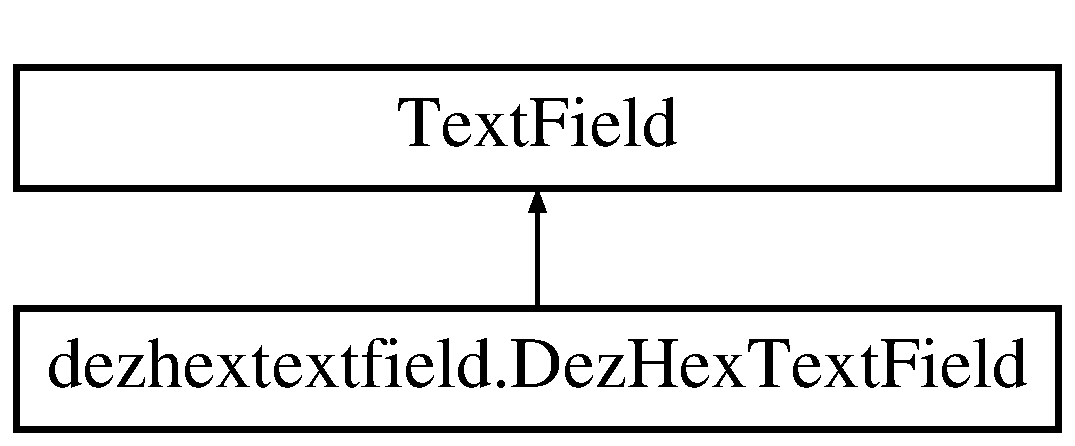
\includegraphics[height=2.000000cm]{classdezhextextfield_1_1_dez_hex_text_field}
\end{center}
\end{figure}
\subsection*{Public Member Functions}
\begin{DoxyCompactItemize}
\item 
void \hyperlink{classdezhextextfield_1_1_dez_hex_text_field_a0ee6264f69424e40d69c03b7b41fb08c}{replace\+Text} (int start, int end, String text)
\item 
void \hyperlink{classdezhextextfield_1_1_dez_hex_text_field_a617d0b9fe256c02dfed2b1a93a66db83}{replace\+Selection} (String text)
\end{DoxyCompactItemize}
\subsection*{Private Member Functions}
\begin{DoxyCompactItemize}
\item 
void \hyperlink{classdezhextextfield_1_1_dez_hex_text_field_a091d736c5cbf7c6aa896539399df3b33}{verify} ()
\end{DoxyCompactItemize}


\subsection{Detailed Description}


Definition at line 4 of file Dez\+Hex\+Text\+Field.\+java.



\subsection{Member Function Documentation}
\mbox{\Hypertarget{classdezhextextfield_1_1_dez_hex_text_field_a617d0b9fe256c02dfed2b1a93a66db83}\label{classdezhextextfield_1_1_dez_hex_text_field_a617d0b9fe256c02dfed2b1a93a66db83}} 
\index{dezhextextfield\+::\+Dez\+Hex\+Text\+Field@{dezhextextfield\+::\+Dez\+Hex\+Text\+Field}!replace\+Selection@{replace\+Selection}}
\index{replace\+Selection@{replace\+Selection}!dezhextextfield\+::\+Dez\+Hex\+Text\+Field@{dezhextextfield\+::\+Dez\+Hex\+Text\+Field}}
\subsubsection{\texorpdfstring{replace\+Selection()}{replaceSelection()}}
{\footnotesize\ttfamily void dezhextextfield.\+Dez\+Hex\+Text\+Field.\+replace\+Selection (\begin{DoxyParamCaption}\item[{String}]{text }\end{DoxyParamCaption})}



Definition at line 15 of file Dez\+Hex\+Text\+Field.\+java.



References dezhextextfield.\+Dez\+Hex\+Text\+Field.\+verify().

\mbox{\Hypertarget{classdezhextextfield_1_1_dez_hex_text_field_a0ee6264f69424e40d69c03b7b41fb08c}\label{classdezhextextfield_1_1_dez_hex_text_field_a0ee6264f69424e40d69c03b7b41fb08c}} 
\index{dezhextextfield\+::\+Dez\+Hex\+Text\+Field@{dezhextextfield\+::\+Dez\+Hex\+Text\+Field}!replace\+Text@{replace\+Text}}
\index{replace\+Text@{replace\+Text}!dezhextextfield\+::\+Dez\+Hex\+Text\+Field@{dezhextextfield\+::\+Dez\+Hex\+Text\+Field}}
\subsubsection{\texorpdfstring{replace\+Text()}{replaceText()}}
{\footnotesize\ttfamily void dezhextextfield.\+Dez\+Hex\+Text\+Field.\+replace\+Text (\begin{DoxyParamCaption}\item[{int}]{start,  }\item[{int}]{end,  }\item[{String}]{text }\end{DoxyParamCaption})}



Definition at line 6 of file Dez\+Hex\+Text\+Field.\+java.



References dezhextextfield.\+Dez\+Hex\+Text\+Field.\+verify().

\mbox{\Hypertarget{classdezhextextfield_1_1_dez_hex_text_field_a091d736c5cbf7c6aa896539399df3b33}\label{classdezhextextfield_1_1_dez_hex_text_field_a091d736c5cbf7c6aa896539399df3b33}} 
\index{dezhextextfield\+::\+Dez\+Hex\+Text\+Field@{dezhextextfield\+::\+Dez\+Hex\+Text\+Field}!verify@{verify}}
\index{verify@{verify}!dezhextextfield\+::\+Dez\+Hex\+Text\+Field@{dezhextextfield\+::\+Dez\+Hex\+Text\+Field}}
\subsubsection{\texorpdfstring{verify()}{verify()}}
{\footnotesize\ttfamily void dezhextextfield.\+Dez\+Hex\+Text\+Field.\+verify (\begin{DoxyParamCaption}{ }\end{DoxyParamCaption})\hspace{0.3cm}{\ttfamily [private]}}



Definition at line 24 of file Dez\+Hex\+Text\+Field.\+java.



Referenced by dezhextextfield.\+Dez\+Hex\+Text\+Field.\+replace\+Selection(), and dezhextextfield.\+Dez\+Hex\+Text\+Field.\+replace\+Text().



The documentation for this class was generated from the following file\+:\begin{DoxyCompactItemize}
\item 
dezhextextfield/\hyperlink{_dez_hex_text_field_8java}{Dez\+Hex\+Text\+Field.\+java}\end{DoxyCompactItemize}

\hypertarget{classdezhex_1_1_gradle_dez_hex}{}\section{dezhex.\+Gradle\+Dez\+Hex Class Reference}
\label{classdezhex_1_1_gradle_dez_hex}\index{dezhex.\+Gradle\+Dez\+Hex@{dezhex.\+Gradle\+Dez\+Hex}}
Inheritance diagram for dezhex.\+Gradle\+Dez\+Hex\+:\begin{figure}[H]
\begin{center}
\leavevmode
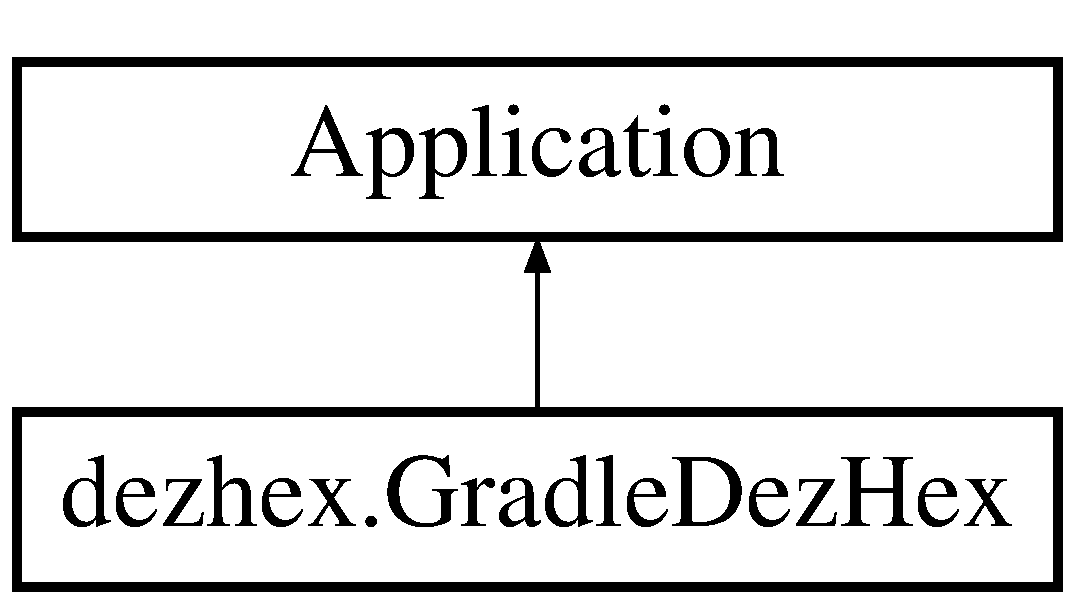
\includegraphics[height=2.000000cm]{classdezhex_1_1_gradle_dez_hex}
\end{center}
\end{figure}
\subsection*{Public Member Functions}
\begin{DoxyCompactItemize}
\item 
void \hyperlink{classdezhex_1_1_gradle_dez_hex_ae0b72fc8103dca55356650ac085d2c7e}{start} (Stage primary\+Stage)  throws Exception 
\end{DoxyCompactItemize}
\subsection*{Static Public Member Functions}
\begin{DoxyCompactItemize}
\item 
static void \hyperlink{classdezhex_1_1_gradle_dez_hex_a5b39f02998d799114ecb4675f64c5453}{main} (String\mbox{[}$\,$\mbox{]} args)
\end{DoxyCompactItemize}


\subsection{Detailed Description}
The class description. 

Definition at line 9 of file Gradle\+Dez\+Hex.\+java.



\subsection{Member Function Documentation}
\mbox{\Hypertarget{classdezhex_1_1_gradle_dez_hex_a5b39f02998d799114ecb4675f64c5453}\label{classdezhex_1_1_gradle_dez_hex_a5b39f02998d799114ecb4675f64c5453}} 
\index{dezhex\+::\+Gradle\+Dez\+Hex@{dezhex\+::\+Gradle\+Dez\+Hex}!main@{main}}
\index{main@{main}!dezhex\+::\+Gradle\+Dez\+Hex@{dezhex\+::\+Gradle\+Dez\+Hex}}
\subsubsection{\texorpdfstring{main()}{main()}}
{\footnotesize\ttfamily static void dezhex.\+Gradle\+Dez\+Hex.\+main (\begin{DoxyParamCaption}\item[{String \mbox{[}$\,$\mbox{]}}]{args }\end{DoxyParamCaption})\hspace{0.3cm}{\ttfamily [static]}}



Definition at line 10 of file Gradle\+Dez\+Hex.\+java.

\mbox{\Hypertarget{classdezhex_1_1_gradle_dez_hex_ae0b72fc8103dca55356650ac085d2c7e}\label{classdezhex_1_1_gradle_dez_hex_ae0b72fc8103dca55356650ac085d2c7e}} 
\index{dezhex\+::\+Gradle\+Dez\+Hex@{dezhex\+::\+Gradle\+Dez\+Hex}!start@{start}}
\index{start@{start}!dezhex\+::\+Gradle\+Dez\+Hex@{dezhex\+::\+Gradle\+Dez\+Hex}}
\subsubsection{\texorpdfstring{start()}{start()}}
{\footnotesize\ttfamily void dezhex.\+Gradle\+Dez\+Hex.\+start (\begin{DoxyParamCaption}\item[{Stage}]{primary\+Stage }\end{DoxyParamCaption}) throws Exception}



Definition at line 16 of file Gradle\+Dez\+Hex.\+java.



The documentation for this class was generated from the following file\+:\begin{DoxyCompactItemize}
\item 
dezhex/\hyperlink{_gradle_dez_hex_8java}{Gradle\+Dez\+Hex.\+java}\end{DoxyCompactItemize}

\hypertarget{classdezhex_1_1_hilfe_fenster}{}\section{dezhex.\+Hilfe\+Fenster Class Reference}
\label{classdezhex_1_1_hilfe_fenster}\index{dezhex.\+Hilfe\+Fenster@{dezhex.\+Hilfe\+Fenster}}
Inheritance diagram for dezhex.\+Hilfe\+Fenster\+:\begin{figure}[H]
\begin{center}
\leavevmode
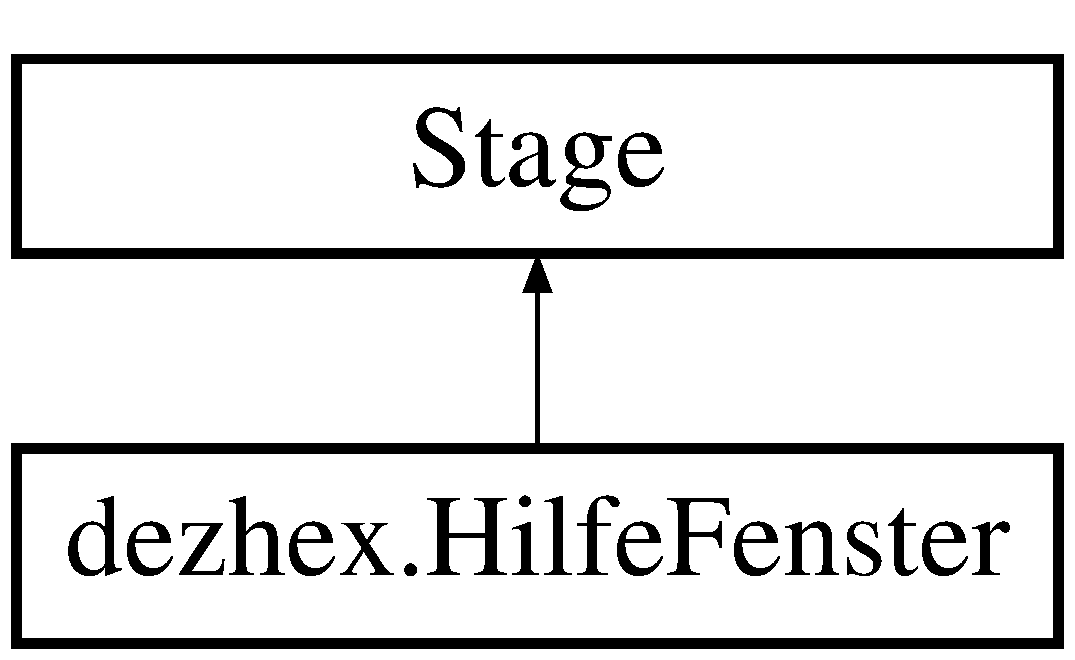
\includegraphics[height=2.000000cm]{classdezhex_1_1_hilfe_fenster}
\end{center}
\end{figure}
\subsection*{Public Member Functions}
\begin{DoxyCompactItemize}
\item 
\hyperlink{classdezhex_1_1_hilfe_fenster_ad24f38e5ef3de17205242d57b7fab65a}{Hilfe\+Fenster} (int auswahl)
\end{DoxyCompactItemize}


\subsection{Detailed Description}


Definition at line 17 of file Hilfe\+Fenster.\+java.



\subsection{Constructor \& Destructor Documentation}
\mbox{\Hypertarget{classdezhex_1_1_hilfe_fenster_ad24f38e5ef3de17205242d57b7fab65a}\label{classdezhex_1_1_hilfe_fenster_ad24f38e5ef3de17205242d57b7fab65a}} 
\index{dezhex\+::\+Hilfe\+Fenster@{dezhex\+::\+Hilfe\+Fenster}!Hilfe\+Fenster@{Hilfe\+Fenster}}
\index{Hilfe\+Fenster@{Hilfe\+Fenster}!dezhex\+::\+Hilfe\+Fenster@{dezhex\+::\+Hilfe\+Fenster}}
\subsubsection{\texorpdfstring{Hilfe\+Fenster()}{HilfeFenster()}}
{\footnotesize\ttfamily dezhex.\+Hilfe\+Fenster.\+Hilfe\+Fenster (\begin{DoxyParamCaption}\item[{int}]{auswahl }\end{DoxyParamCaption})}



Definition at line 24 of file Hilfe\+Fenster.\+java.



The documentation for this class was generated from the following file\+:\begin{DoxyCompactItemize}
\item 
dezhex/\hyperlink{_hilfe_fenster_8java}{Hilfe\+Fenster.\+java}\end{DoxyCompactItemize}

\chapter{File Documentation}
\hypertarget{_dez_hex_controller_8java}{}\section{dezhex/\+Dez\+Hex\+Controller.java File Reference}
\label{_dez_hex_controller_8java}\index{dezhex/\+Dez\+Hex\+Controller.\+java@{dezhex/\+Dez\+Hex\+Controller.\+java}}
\subsection*{Classes}
\begin{DoxyCompactItemize}
\item 
class \hyperlink{classdezhex_1_1_dez_hex_controller}{dezhex.\+Dez\+Hex\+Controller}
\end{DoxyCompactItemize}
\subsection*{Packages}
\begin{DoxyCompactItemize}
\item 
package \hyperlink{namespacedezhex}{dezhex}
\end{DoxyCompactItemize}

\hypertarget{_gradle_dez_hex_8java}{}\section{dezhex/\+Gradle\+Dez\+Hex.java File Reference}
\label{_gradle_dez_hex_8java}\index{dezhex/\+Gradle\+Dez\+Hex.\+java@{dezhex/\+Gradle\+Dez\+Hex.\+java}}
\subsection*{Classes}
\begin{DoxyCompactItemize}
\item 
class \hyperlink{classdezhex_1_1_gradle_dez_hex}{dezhex.\+Gradle\+Dez\+Hex}
\end{DoxyCompactItemize}
\subsection*{Packages}
\begin{DoxyCompactItemize}
\item 
package \hyperlink{namespacedezhex}{dezhex}
\end{DoxyCompactItemize}

\hypertarget{_hilfe_fenster_8java}{}\section{dezhex/\+Hilfe\+Fenster.java File Reference}
\label{_hilfe_fenster_8java}\index{dezhex/\+Hilfe\+Fenster.\+java@{dezhex/\+Hilfe\+Fenster.\+java}}
\subsection*{Classes}
\begin{DoxyCompactItemize}
\item 
class \hyperlink{classdezhex_1_1_hilfe_fenster}{dezhex.\+Hilfe\+Fenster}
\end{DoxyCompactItemize}
\subsection*{Packages}
\begin{DoxyCompactItemize}
\item 
package \hyperlink{namespacedezhex}{dezhex}
\end{DoxyCompactItemize}

\hypertarget{_dez_hex_text_field_8java}{}\section{dezhextextfield/\+Dez\+Hex\+Text\+Field.java File Reference}
\label{_dez_hex_text_field_8java}\index{dezhextextfield/\+Dez\+Hex\+Text\+Field.\+java@{dezhextextfield/\+Dez\+Hex\+Text\+Field.\+java}}
\subsection*{Classes}
\begin{DoxyCompactItemize}
\item 
class \hyperlink{classdezhextextfield_1_1_dez_hex_text_field}{dezhextextfield.\+Dez\+Hex\+Text\+Field}
\end{DoxyCompactItemize}
\subsection*{Packages}
\begin{DoxyCompactItemize}
\item 
package \hyperlink{namespacedezhextextfield}{dezhextextfield}
\end{DoxyCompactItemize}

%--- End generated contents ---

% Index
\backmatter
\newpage
\phantomsection
\clearemptydoublepage
\addcontentsline{toc}{chapter}{Index}
\printindex

\end{document}
